% ---------------------------------------------------------------------
% HEADER
% Formålet med å legge header til et eget dokument er å garantere at
% oppsettet av dokumentene er likt for alle løsningsforslagene.
% I headeren skjer følgende:
% (1) Dokumentet blir startet
% (2) Pakker blir importert
% ---------------------------------------------------------------------
\input{../../header.tex}


% ---------------------------------------------------------------------
% DOKUMENTVARIABLER
% ---------------------------------------------------------------------
\newcommand{\fagkode}{R1}
\newcommand{\semesteraar}{våren 2018}
\newcommand{\forfatter}{Anita G.}
\newcommand{\dokumenttittel}{Løsningsforslag -- Eksamen \fagkode, \semesteraar}

\usepackage{siunitx}


% Set til 'true' og oppgi logo dersom du vil bruke en logo
\newboolean{bruklogo}
\setboolean{bruklogo}{false}
\newcommand{\logonavn}{}



% ---------------------------------------------------------------------
% SETUP
% Formålet med å legge setup til et eget dokument å garantere at headers,
% footers, og øverste del av dokumentet er likt for alle
% løsningsforslagene.
% ---------------------------------------------------------------------
\input{../../setup.tex}


% ---------------------------------------------------------------------
% DOKUMENTSTART - Skriv løsningsforslaget nedenfor
% ---------------------------------------------------------------------	
\section*{Del 1 - uten hjelpemidler}
\subsection*{Oppgave 1}
\begin{easylist}[enumerate]
	\ListProperties(Style2*=,Numbers=a,Numbers1=l,FinalMark={)})
	# Vi skal derivere $f(x) = x^4 - x +2$. Vi bruker regelen $f(x) = x^n \Rightarrow f'(x) = nx^{n-1}$. Vi får da at $f'(x) = 4x^3 - 1$.
	
	# Her ser vi at funksjonen g er sammensatt av to funksjoner som er multiplisert sammen, nemlig $x^3$ og $\ln(x)$. Vi bruker derfor produktregelen: $f(x) = uv \Rightarrow f'(x) = u'v + uv'$. Vi får da 
	\begin{equation*}
		\begin{aligned}
			g'(x) &= 3x^2 \cdot \ln(x) + x^3 \cdot \frac{1}{x}\\
					&= 3x^2\ln(x) + x^2\\
					&= x^2(3\ln(x)+1)\\
		\end{aligned}
	\end{equation*}
	
	# Her får vi bruk for kjerneregelen, der vi velger at kjernen vår er $u = 2x^2 + x$. Vi har at 
	\begin{equation*}
		\begin{aligned}
				h(x) = e^{u(x)} \Rightarrow h'(x) &= (e^{u(x)})' \cdot u'(x) \\
																  &= e^{u(x)} \cdot (4x + 1) \\
																  &= (4x +1)e^{2x^2 + x}
		\end{aligned}
	\end{equation*}
\end{easylist}


\subsection*{Oppgave 2}
\begin{easylist}[enumerate]
	\ListProperties(Style2*=,Numbers=a,Numbers1=l,FinalMark={)})
	# 
	\begin{equation*}
		\frac{1}{2x-2} + \frac{2}{x-3} - \frac{x-2}{x^2 - 4x +3}
	\end{equation*}
	Først faktoriserer vi nevnerene for å finne ut hva fellesnevneren til brøkene er. Nevneren i det første leddet faktoriseres slik: $2x-2 = 2(x-1)$. Nevneren i andre ledd kan ikke faktoriseres, mens nevneren i det tredje leddet kan vi faktorisere for eksempel ved bruk av abc-formelen. Etter faktoriseringen ser uttrykket ut slik
	
	\begin{equation*}
		\begin{aligned}
			\frac{1}{2(x-1)} + \frac{2}{x-3} - \frac{x-2}{(x-1)(x-3)}
		\end{aligned}
	\end{equation*}
	
	Vi ser dermed at fellesnevneren er $2(x-1)(x-3)$. Vi ganger første ledd med $(x-3)$ i både teller og nevner, andre ledd med $2(x-1)$ og tredje ledd med $2$.
	
	\begin{equation*}
		\begin{aligned}
			&\frac{1(x-3)}{2(x-1)(x-3)} + \frac{2 \cdot 2(x-1)}{2(x-1)(x-3)} - \frac{2(x-3)}{2(x-1)(x-3)} \\
			& = \frac{x - 3 +4x - 4 - 2x + 6}{2(x-1)(x-3)} \\
													& = \frac{x-1}{2(x-1)(x-3)}\\
													& = \frac{1}{2(x-3)}
		\end{aligned}
	\end{equation*}
	
	# Her må vi ta i bruk logaritmesetningene. Disse er: $\ln(ab) = \ln(a) + \ln(b)$, $\ln\left(\frac{a}{b}\right) = \ln(a) - \ln(b)$ og $\ln(a^x) = x \cdot \ln(a)$.
	\begin{equation*}
		\begin{aligned}
		&2\ln(x\cdot y^3) - \frac{1}{2} \ln \left (\frac{x^4}{y^2} \right) \\
		& = 2(\ln(x) + \ln(y^3) - \frac{1}{2}(\ln(x^4) - \ln(y^2)) \\
		& = 2(\ln(x) + 3\ln(y)) - \frac{1}{2}(4\ln(x) - 2\ln(y))\\
		& = 2\ln(x) + 6\ln(y) - 2\ln(x) + \ln(y)\\
		& = \answer{7\ln(y)}
		\end{aligned}
	\end{equation*}
	
\end{easylist}

\subsection*{Oppgave 3}

\begin{easylist}[enumerate]
	\ListProperties(Style2*=,Numbers=a,Numbers1=l,FinalMark={)})
	# Vektoren mellom to punkter $(x_1,y_1)$ og $(x_2,y_2)$ er gitt ved $[x_2 - x_1, y_2 -y_1]$. Vi får da: \newline
	$\vec{AB} = [-1-(-2), -3-(-1)] = [1,-2]$\newline
	$\vec{BC} = [3-(-1),-1-(-3)] = [4,2]$
	
	# Vi har at de to vektorene står vinkelrett på hverandre dersom $\vec{AB} \cdot \vec{BC} = 0$\newline
	$\vec{AB} \cdot \vec{BC} = [1,-2] \cdot [4,2] = 1 \cdot 4 + (-2) \cdot 2 = 4 + (-4) = 0$
	\newline \newline
	Vektorene står vinkelrett på hverandre.
	
	# Vektorene $\vec{CD}$ og $\vec{AB}$ er parallelle dersom $\vec{CD} = k \cdot \vec{AB}$ der $k$ er et tall. Vi finner først $\vec{CD}$ på samme måte som vi fant vektorene i oppgave a. \newline
	$\vec{CD} = [t-3,t^2 + 2- (-1)] = [t-3,t^2 + 3]$\newline \newline
	\begin{equation*}
		\begin{aligned}
		\vec{CD} & = k \cdot \vec{AB}\\
		[t-3,t^2 + 3] & = k \cdot [1,-2] &  = [k,-2k]\\
		\end{aligned}
	\end{equation*}
	
	For at to vektorer skal være like må x-koordinatene være like hverandre og y-koordinatene være like hverandre i de to vektorene. Vi får altså to likninger med to ukjente: 
	
	\begin{equation*}
		\begin{aligned}
		t-3 = k &\:\:\: \vee & t^2 + 3 = -2k \\
		\end{aligned}
	\end{equation*}
	
	Likning nr 1 gir oss et uttrykk for $k$. Dette setter vi inn for $k$ i likning nr 2 og løser for $t$.
	
	\begin{equation*}
		\begin{aligned}
			&t^2 + 3  = -2(t-3)\\
			&t^2 + 3  = -2t + 6\\
			&t^2 +2t -3 = 0   \\ \\
			&\textnormal{vi bruker abc-formelen og får}\\
			&t = 1 \:\:\: eller \:\:\: t=-3
		\end{aligned}
	\end{equation*}
	
	Vi har altså at $\vec{CD}$ og $\vec{AB}$ er parallelle hvis $t = 1$ eller hvis $t = -3$.
	
\end{easylist}

\section*{Oppgave 4}
\begin{easylist}[enumerate]
	\ListProperties(Style2*=,Numbers=a,Numbers1=l,FinalMark={)})
	
	# En divisjon $P(x) : (x-a)$, der $P(x)$ er et polynom, går opp dersom $P(a) = 0$. Vi må altså sjekke for hvilke verdier av k som gjør at $f(1)= 0$.\newline
	
	\begin{equation*}
		\begin{aligned}
		f(1) = 1^3 + k \cdot 1 + 12 &= 0 \\
		1+k+12 & =0 \\
		k + 13 & = 0 \\
		k & = -13 
		\end{aligned}
	\end{equation*}
	
	# Vi har nå at $f(x) = x^3 - 13x + 12$. Vi vet at $f(x)$ er delelig med $(x-1)$, derfor gjør vi en polynomdivisjon med dette for å faktorisere $f$. Vi vil få et andregradspolynom etter polynomdivisjonen som vi kan faktorisere videre ved hjelp av abc-formelen. \newline
	\polylongdiv{x^3 -13x+12}{x - 1} \\ \newline
	
	Ved hjelp av abc-formelen får vi at $(x^2 + x -12 )$ kan faktoriseres til $(x+4)(x-3)$. Når vi nå setter sammen alle de lineære faktorene vi har funnet, har vi at $f(x)$ kan faktoriseres slik: $f(x) = x^3 - 13x + 12 = \answer{(x-1)(x+4)(x-3)}$.
	
	# $$\frac{x^2 + x -12}{x-1}$$
	Fra forrige oppgave vet vi at telleren kan faktoriseres til $(x+4)(x-3)$, som vil si at vi kan skrive brøken som $$\frac{(x+4)(x-3)}{x-1}$$
	
	Vi lager fortegnsskjema. 
	\begin{figure}[ht!]
		\centering
		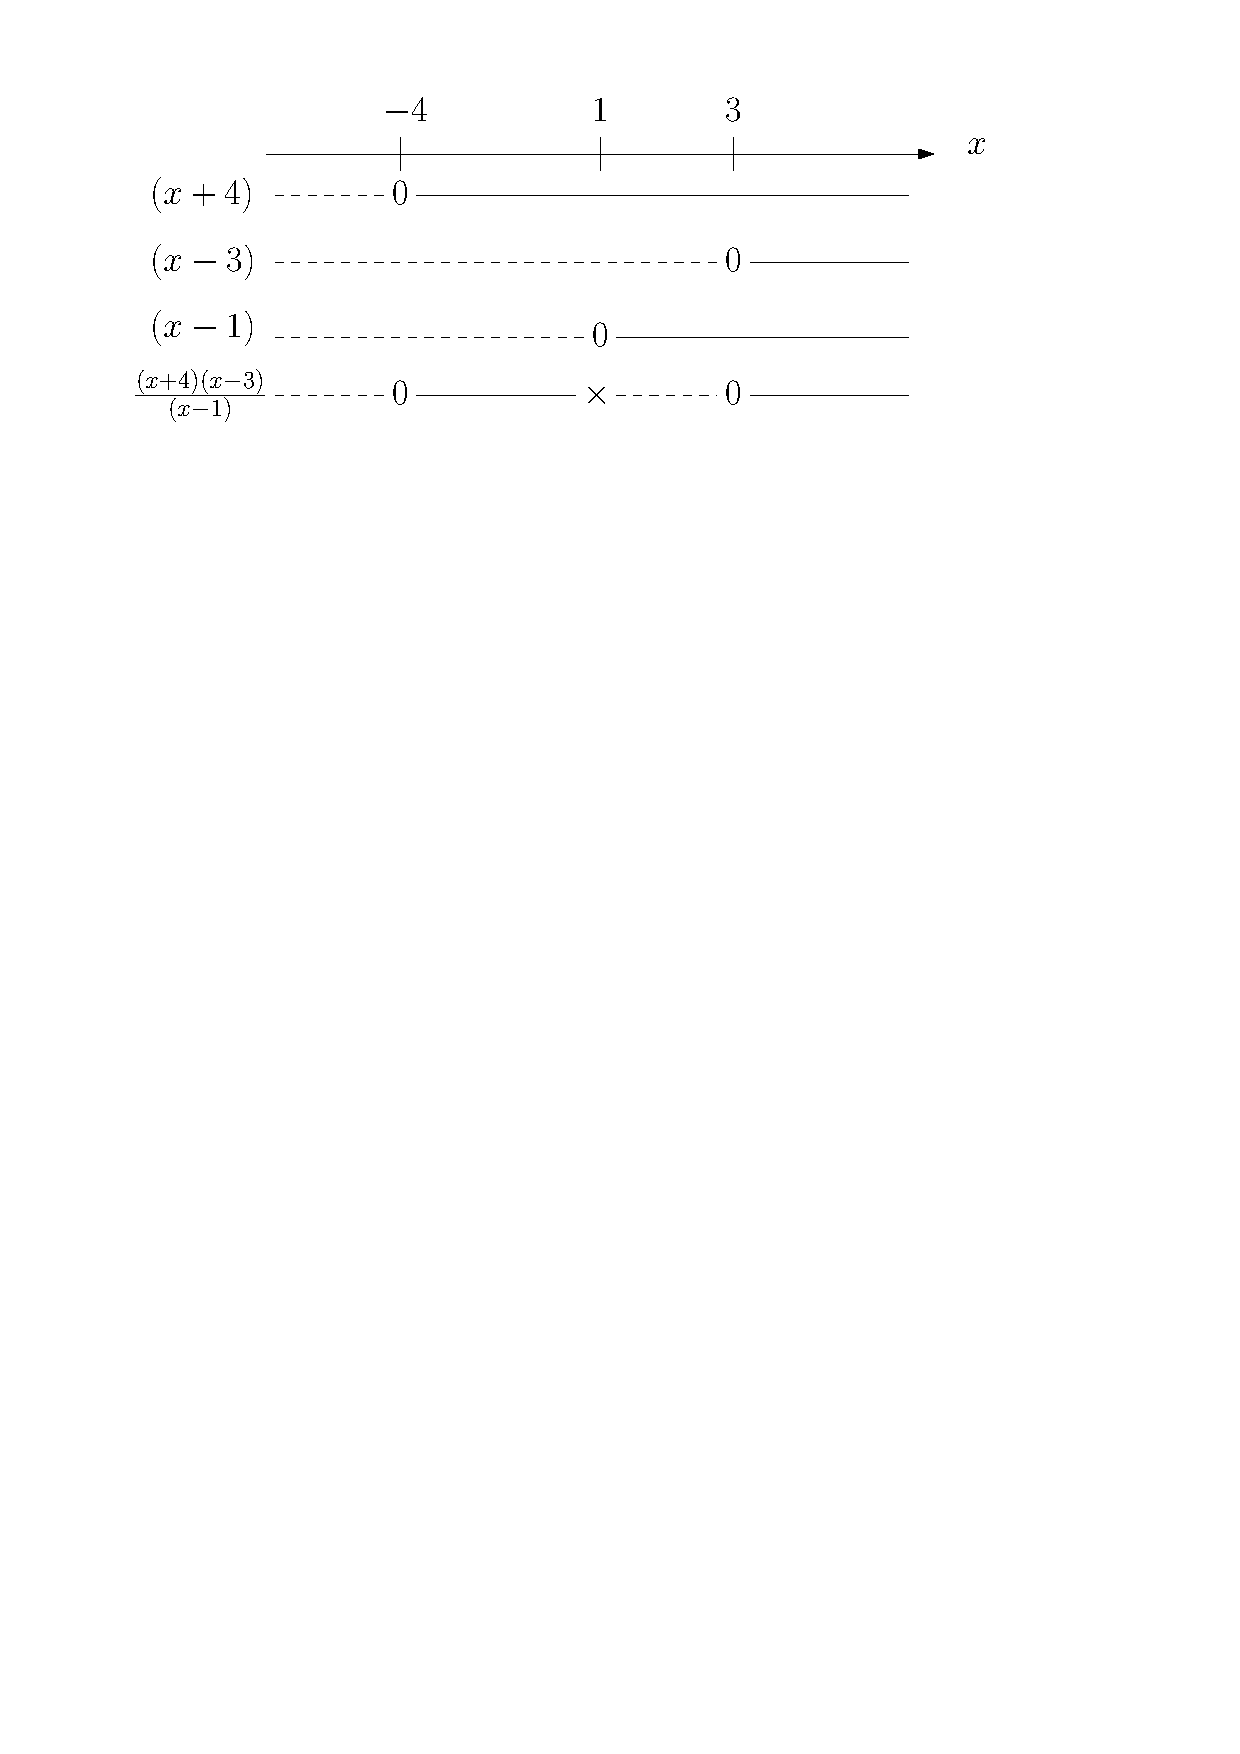
\includegraphics[width=0.85\linewidth]{figs/del1_oppg4c.pdf}
		\label{fig:del1_oppg4c}
	\end{figure}
	
	Vi ser dermed at $$\frac{(x+4)(x-3)}{x-1} \geq 0$$ når \answer{$-4 \leq x < 1$ og når $x \geq 3$}.
	
\end{easylist}

\subsection*{Oppgave 5}

\begin{easylist}[enumerate]
	\ListProperties(Style2*=,Numbers=a,Numbers1=l,FinalMark={)})
	
	
	# Vi bruker i denne oppgaven produktsetningen. Vi skal finne sannsynligheten for at laderen kommer fra leverandør A \textit{og} at den er defekt, altså sannsynligheten $P(\textnormal{fra leverandør A} \: \cap \: \textnormal{defekt})$.
	
	\begin{equation*}
		\begin{aligned}
			P(\textnormal{fra leverandør A} \: \cap \: \textnormal{defekt}) & = P(\textnormal{fra leverandør A}) \cdot P(\textnormal{defekt}  \: | \: \textnormal{fra leverandør A}) \\
			& = 0.4 \cdot 0.03 \\
			& = 0.012
		\end{aligned}
	\end{equation*}
	
	\answer{Sannsynligheten for at laderen er fra leverandør A og er defekt er 1.2 \%.}
	
	# For å bestemme sannsynligheten for at en lader som er defekt kommer fra leverandør A, kan vi bruke Bayes' setning og setningen om total sannsynlighet. 
	
	Bayes' setning i dette tilfellet blir 
	
	\begin{equation*}
		\begin{aligned}
			P(\textnormal{fra leverandør A} \: | \:  \textnormal{defekt}) &= \frac{P(\textnormal{fra leverandør A}) \cdot P(\textnormal{defekt} \: | \: \textnormal{fra leverandør A})}{P(\textnormal{defekt})} \\
		\end{aligned}
	\end{equation*}

	Men for å kunne bruke denne formelen er vi nødt til å finne ut hva $P(defekt)$ er. Det gjør vi ved hjelp av setningen om total sannsynlighet.
	
	\begin{equation*}
		\begin{aligned}
			P(\textnormal{defekt}) & = P(\textnormal{fra leverandør A}) \cdot P(\textnormal{defekt} \: | \: \textnormal{fra leverandør A}) \\
			& + P(\textnormal{fra leverandør B}) \cdot P(\textnormal{defekt} \: | \: \textnormal{fra leverandør B})
			& = 0.4 \cdot 0.03 + 0.6 \cdot 0.02 \\
			& = 0.024
		\end{aligned}
	\end{equation*}
	
	Nå setter vi dette inn i nevneren i Bayes' setning og får:
	
	\begin{equation*}
		\begin{aligned}
			P(\textnormal{fra leverandør A} \: | \:  \textnormal{defekt}) &= \frac{P(\textnormal{fra leverandør A}) \cdot P(\textnormal{defekt} \: | \: \textnormal{fra leverandør A})}{P(\textnormal{defekt})} \\
			& = \frac{0.04 \cdot 0.03}{0.024} \\
			& = \frac{0.012}{0.024} \\
			& = \frac{1}{2}
		\end{aligned}
	\end{equation*}	
	
	\answer{Sannsynligheten for at en defekt lader er fra leverandør A er 50 \%}
\end{easylist}


	
\subsection*{Oppgave 6}

\begin{easylist}[enumerate]
	\ListProperties(Style2*=,Numbers=a,Numbers1=l,FinalMark={)})
	
	# Vi finner nullpunktene til en funksjon ved å sette funksjonsuttrykket lik $0$: $f(x) = 0$, og løser likningen.
	
	\begin{equation*}
	\begin{aligned}
		e^{2x} - 4e^{x} + 3 &= 0 \qquad \textnormal{vi setter $e^x = u$}\\ 
		u^2 - 4u + 3 &= 0\\	
	\end{aligned}
	\end{equation*}
	
	Vi bruker abc-formelen for å løse denne andregradslikningen, og får at $u = 3$ og $u = 1$. Dette gir oss to likninger som vi nå kan løse for $x$.
	
	\begin{equation*}
		\begin{aligned}
		u = 3 & \qquad u = 1 \\
		e^x = 3 & \qquad e^x = 1 \\
		\ln e^x = \ln 1 & \qquad \ln e^x = \ln 3\\
		x = 0 & \qquad x = \ln 3 \approx 1.10
		\end{aligned}
	\end{equation*}
	
	Nullpunktene til $f(x)$ er altså $	\answer{x = 0}$ og $\answer{x = \ln 3 \approx 1.10}$.
	
	# For å bestemme eventuelle topp- og bunnpunkter til funksjonen, deriverer vi funksjonen og ser når den deriverte er lik $0$. Det er blant løsningene vi får til $f'(x) = 0$, vi vil finne de eventuelle topp- og bunnpunktene.
	
	\begin{equation*}
		\begin{aligned}
		f'(x) &= 2e^{2x} - 4e^x \\
		& = 2e^x(e^x - 2)
		\end{aligned}
	\end{equation*}
	
	Så løser vi likningen $f'(x) = 0$
	
	\begin{equation*}
		\begin{aligned}
		f'(x) & = 0 \\
		2e^x(e^x - 2) & = 0 \qquad \textnormal{$2e^x > 0$ alltid, så vi får}\\
		e^x - 2 & = 0 \\
		e^x & = 2 \\
		\ln e^x &=  \ln 2\\
		x & = \ln 2
		\end{aligned}
	\end{equation*}
	
	Vi lager fortegnslinje for å sjekke om dette punktet er et topp- eller bunnpunkt, eller ingen av delene.
	
	\begin{figure}[ht!]
		\centering
		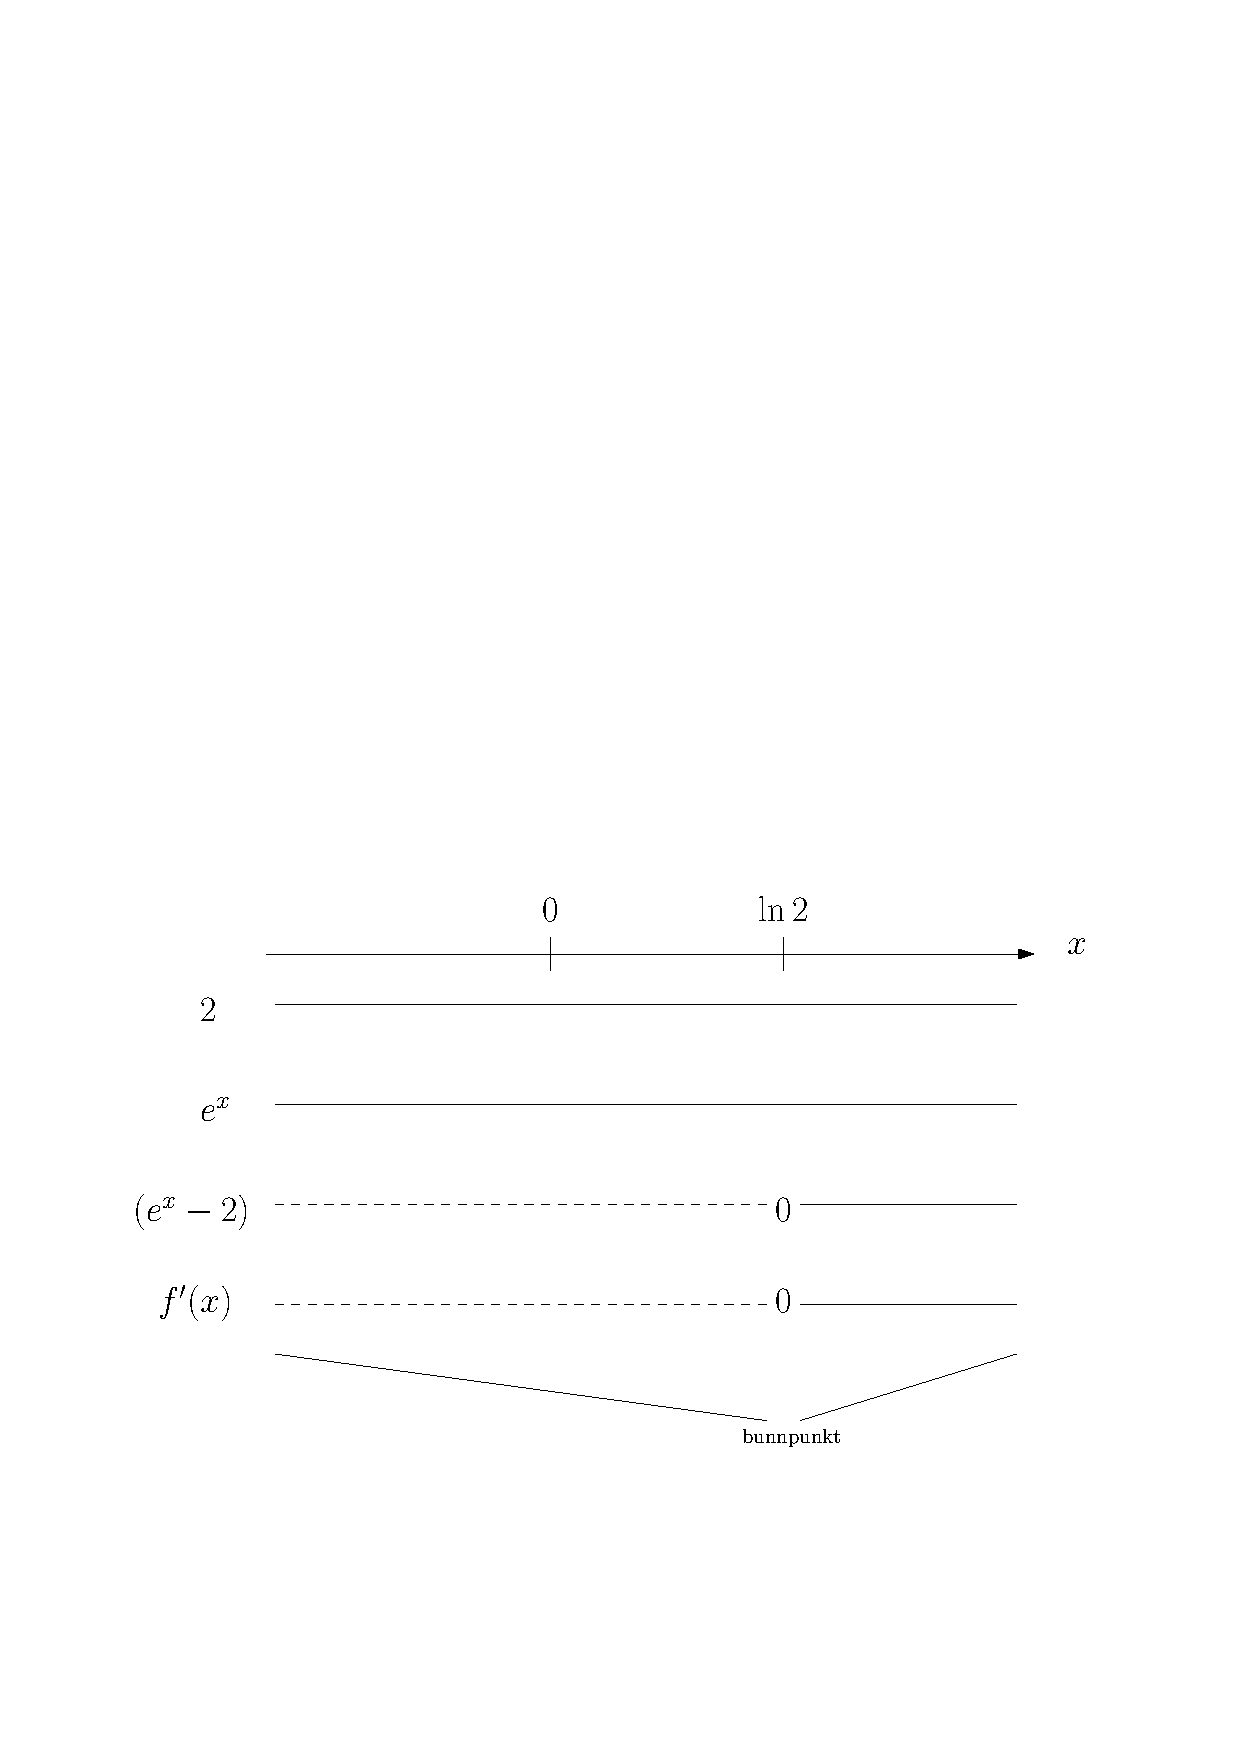
\includegraphics[width=0.85\linewidth]{figs/del1_oppg6b.pdf}
		\label{fig:del1_oppg6b}
	\end{figure}
	
	Vi ser av fortegnslinjen at vi har et bunnpunkt i $x = \ln 2$. Funksjonsverdien for denne $x$-verdien er
	
	\begin{equation*}
		\begin{aligned}
		f(\ln 2) & = e^{2\ln2} - 4e^{\ln 2} + 3\\
		& = e^{\ln 2^2} - 4e^{\ln 2} + 3 \\
		& = 4 - 8 + 3 \\
		& = -1
		\end{aligned}
	\end{equation*}
	
	Bunnpunktet er altså $\answer{(\ln 2, -1)}$.
	
	
	# Når vi skal bestemme eventuelle vendepunkt, kan vi undersøke hvor den dobbeltderiverte av funksjonen endrer fortegn. Vi deriverer derfor den deriverte vi fant i forrige deloppgave. 
	
	\begin{equation*}
		\begin{aligned}
		f''(x) & = 4e^{2x} - 4e^x \\
		& = 4e^x(e^x -1)
		\end{aligned}
	\end{equation*}
	
	Deretter setter vi den dobbeltderiverte lik $0$, og lager igjen fortegnslinje som i oppgaven over.
	
	\begin{equation*}
		\begin{aligned}
		f''(x) & = 0 \\
		4e^x(e^x-1) & = 0 \qquad \textnormal{$4e^x > 0$ alltid, så vi får}\\ 
		e^x -1 & = 0 \\
		e^x & = 1 \\
		\ln e^x & = \ln 1 \\
		x & = 0
		\end{aligned}
	\end{equation*}
	
	Fortegnslinjen vil se slik ut:
	
	\begin{figure}[ht!]
		\centering
		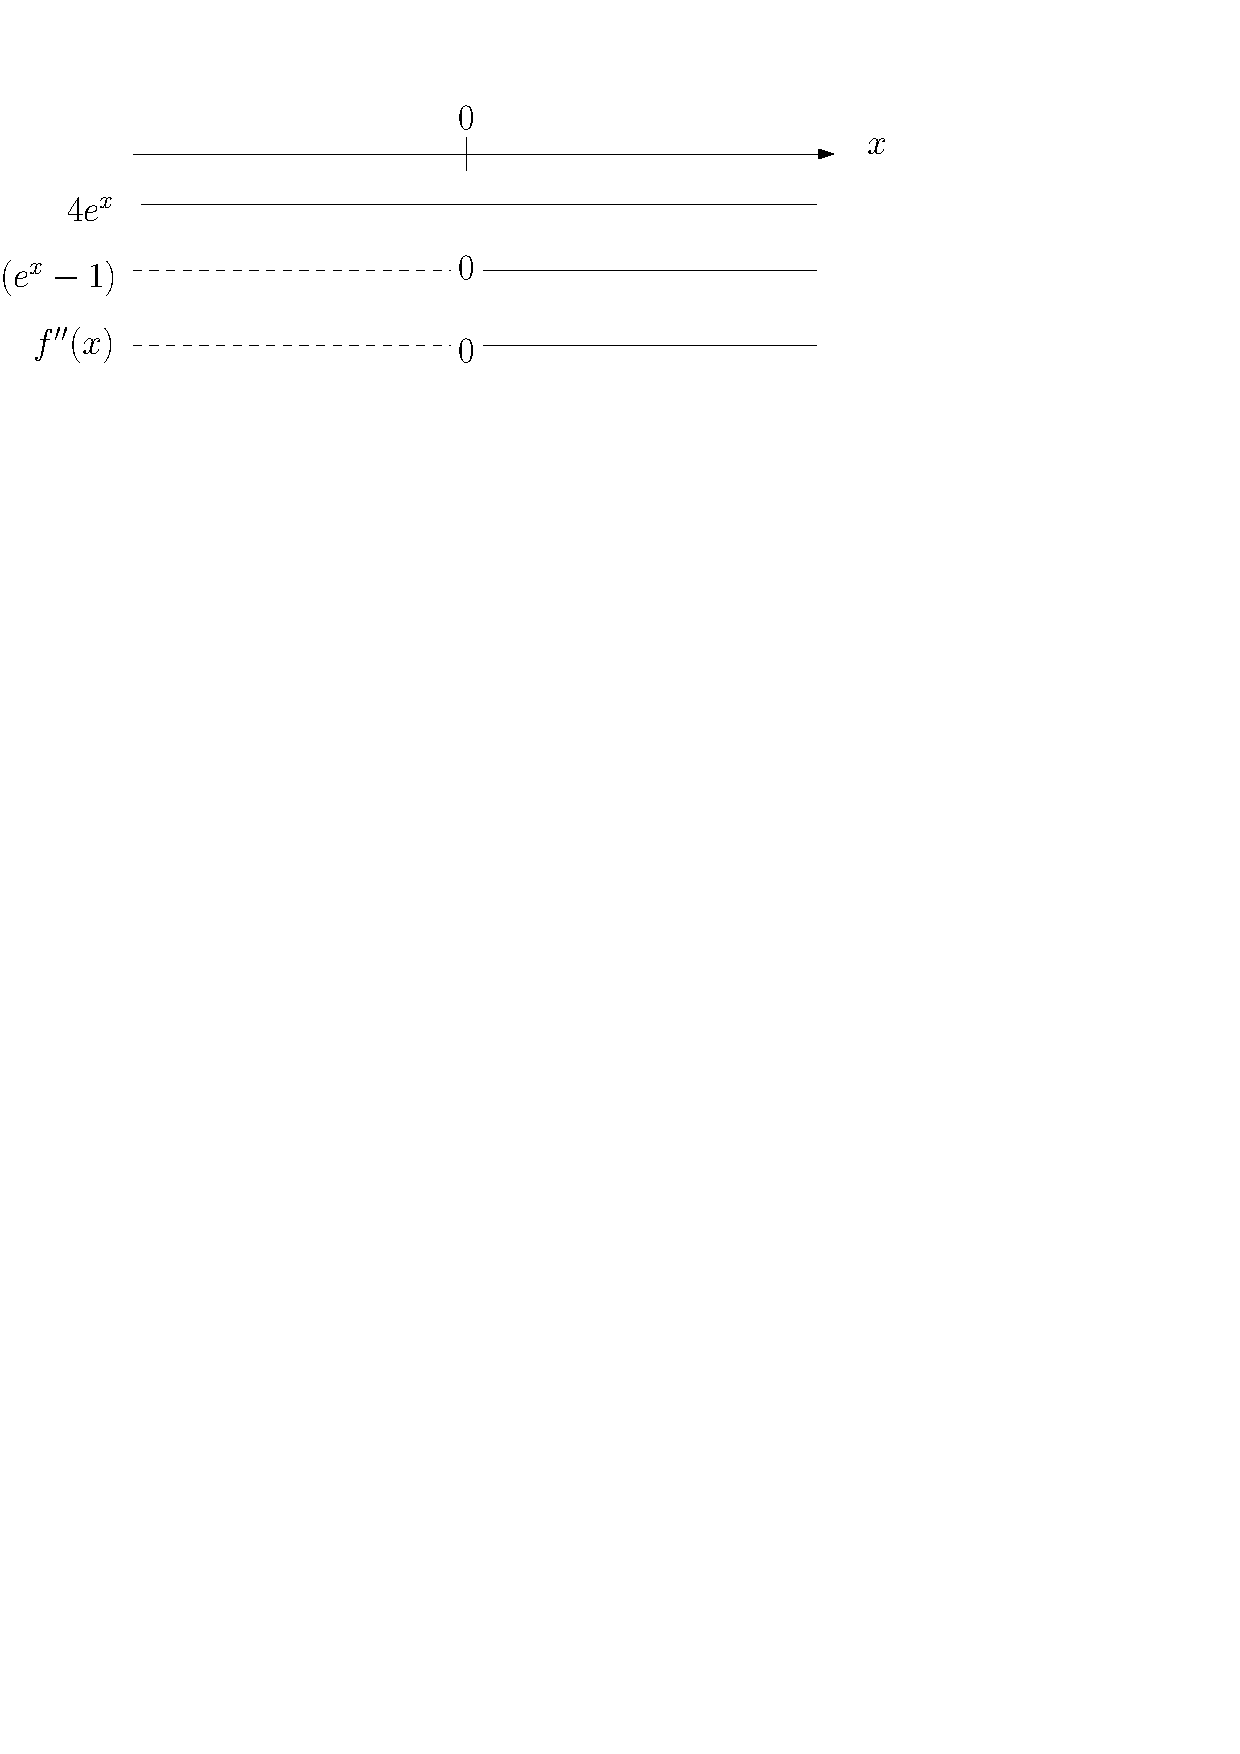
\includegraphics[width=0.85\linewidth]{figs/del1_oppg6c.pdf}
		\label{fig:del1_oppg6c}
	\end{figure}
	
	Vi ser altså at den dobbeltderiverte skifter fortegn når $x=0$. Den tilhørende funksjonsverdien er: 
	
	\begin{equation*}
	\begin{aligned}
	f(0) & = e^{2 \cdot 0} - 4e^0 + 3\\
	& = 1 -4 +3\\
	& = 0\\
	\end{aligned}
	\end{equation*}	
	
	Vendepunktet for funksjonen er altså i punktet $\answer{(0,0)}$.
	
	# Når vi lager en skisse av grafen til funksjonen, er det veldig lurt å tegne inn de punktene vi har funnet i oppgavene over. Disse punktene gir oss god informasjon om hvordan grafen omtrent kan se ut. 
	
	\begin{figure}[ht!]
		\centering
		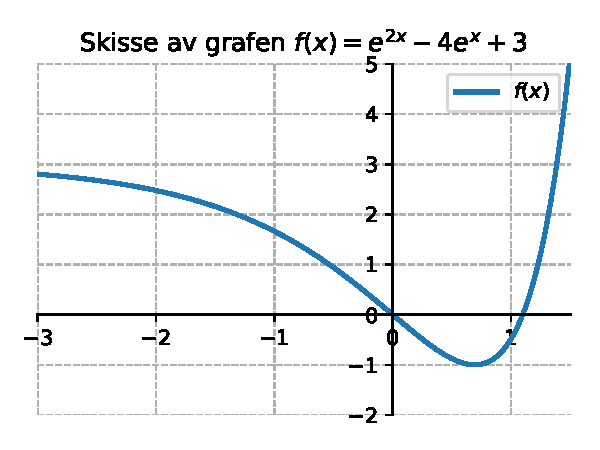
\includegraphics[width = 0.85\linewidth]{figs/del1_oppg6d.pdf}
		\label{fig:del1_oppg6d}
	\end{figure}
	
\end{easylist}

\subsection*{Oppgave 7}

\begin{easylist}[enumerate]
	\ListProperties(Style2*=,Numbers=a,Numbers1=l,FinalMark={)})
	
	# En måte å vise at trekantene er formlike på, er å sjekke at forholdet mellom samsvarende sider er det samme. 
	
	\begin{figure}[ht!]
		\centering
		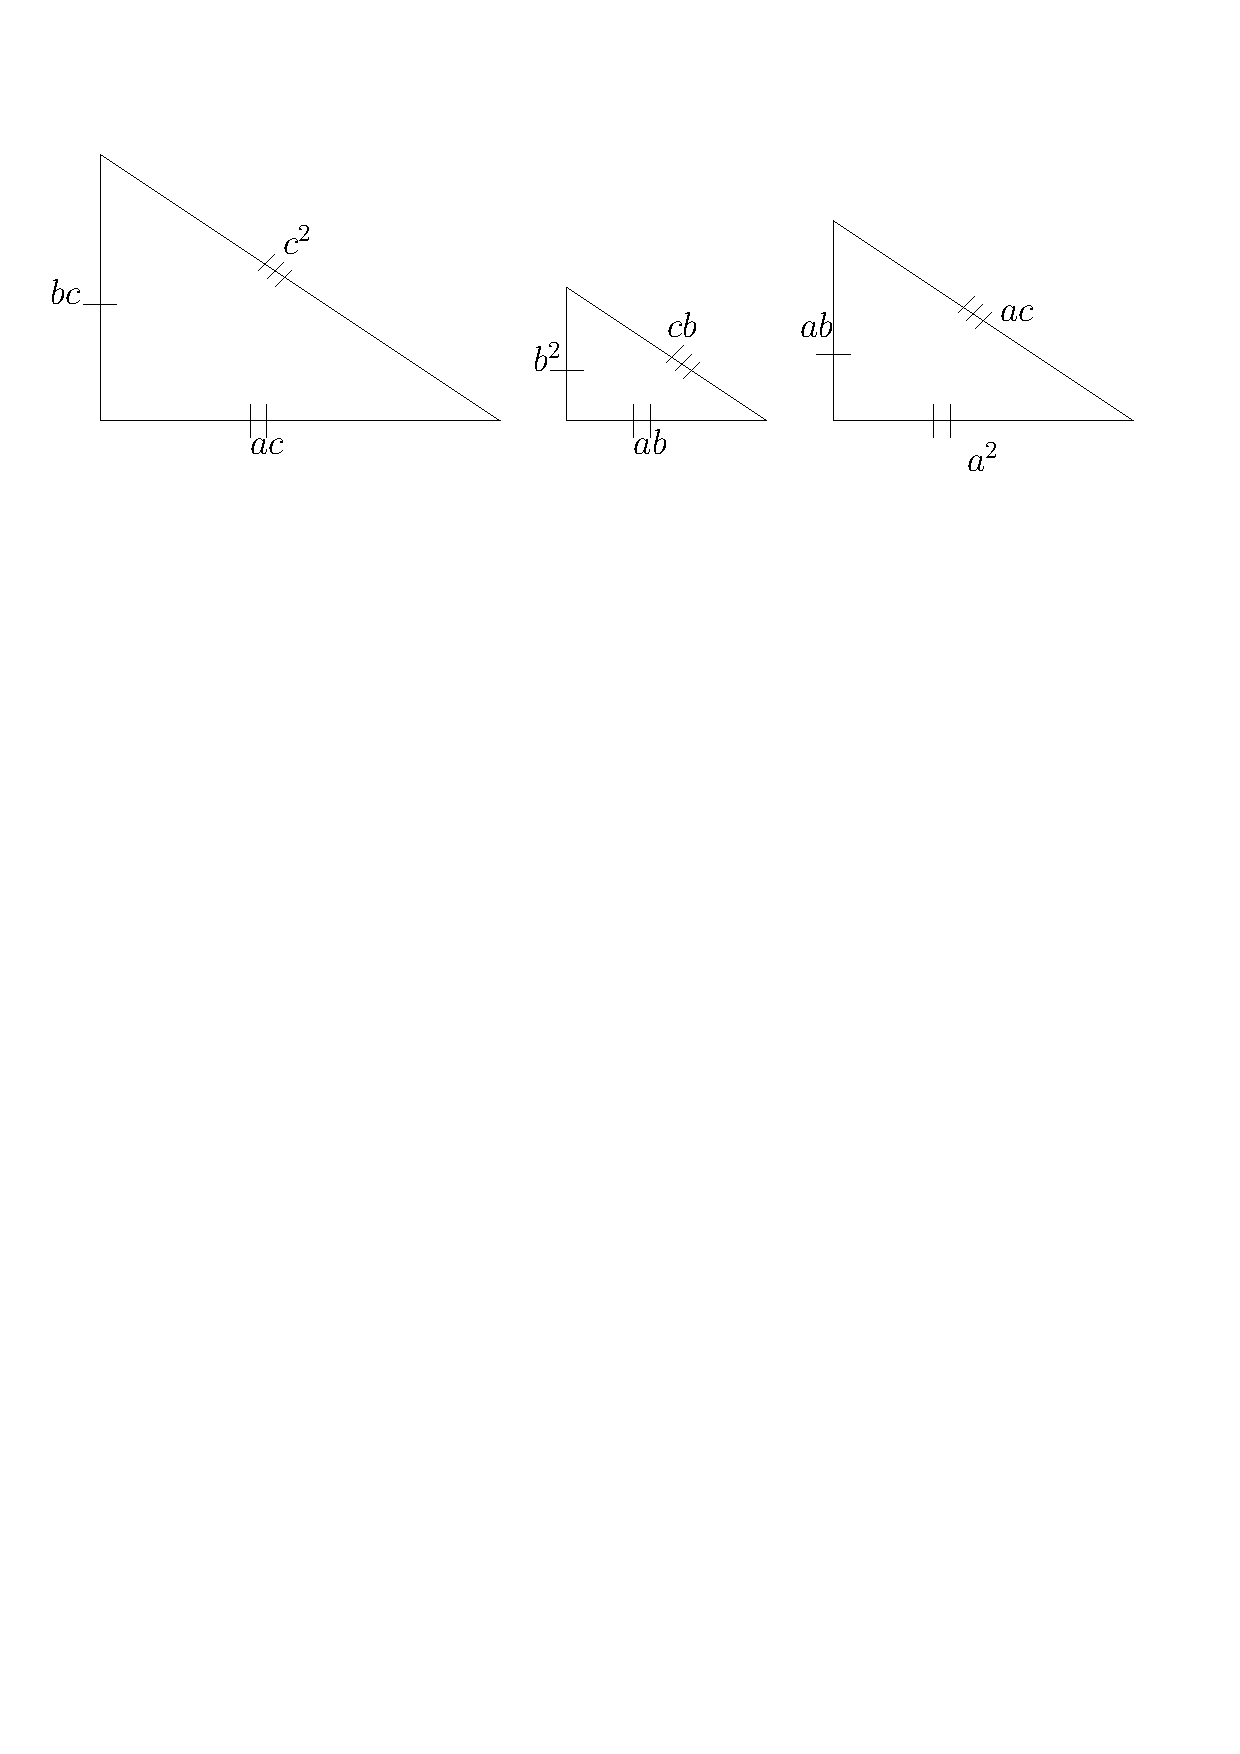
\includegraphics[width = 0.85\linewidth]{figs/del1_oppg7a.pdf}
		\label{fig:del1_oppg7a}
	\end{figure}	
	
		Vi starter med å vise at trekant 1 og 2 er formlike. Forholdet mellom de formlike sidene er:
		
	
	\begin{equation*}
		\begin{aligned}
			\frac{bc}{b^2} & = \frac{c}{b} \\
			\frac{ac}{ab} & = \frac{c}{b} \\
			\frac{c^2}{cb} & = \frac{c}{b} \\			
		\end{aligned}
	\end{equation*}
	
	Deretter sjekker vi om trekant 2 og 3 er formlike
	
	\begin{equation*}
		\begin{aligned}
			\frac{b^2}{ab} & = \frac{b}{a} \\
			\frac{ab}{a^2} & = \frac{b}{a} \\
			\frac{cb}{ac} & = \frac{b}{a} \\			
		\end{aligned}
	\end{equation*}
	
	Vi ser altså at trekant 1 er formlik med trekant 2 og at trekant 2 er formlik med trekant 3. Da må også trekant 1 og 3 være formlike. 
	
	# For å vise at punktene E, D og C ligger på en rett linje, må vi vise at $\angle ADE + \angle BDC = \ang{180} $. Siden de tre trekantene er formlike, vet vi at samsvarende vinkler er like store. Vi vet også at $\angle ADB = \ang{90}$, så det gjenstår å vise at $\angle ADE + \angle BDC = \ang{90}$.
	
	Dette gjør vi ved å trekke to hjelpelinjer som vist på figuren nedenfor. Vi vet at to parallelle linjer som skjæres av samme linje danner samsvarende vinkler. I tillegg får vi toppvinkler. Derfor vet vi at $\angle BAD$ er samsvarende vinkel med $\angle ADE$, som vil si at disse to vinklene er like store. Vi får samme tilfelle for $\angle ABD$. Denne er samsvarende med vinkel $\angle BDC$, altså er disse to vinklene også like store.
	
	\begin{figure}[htbp]
		\centering
		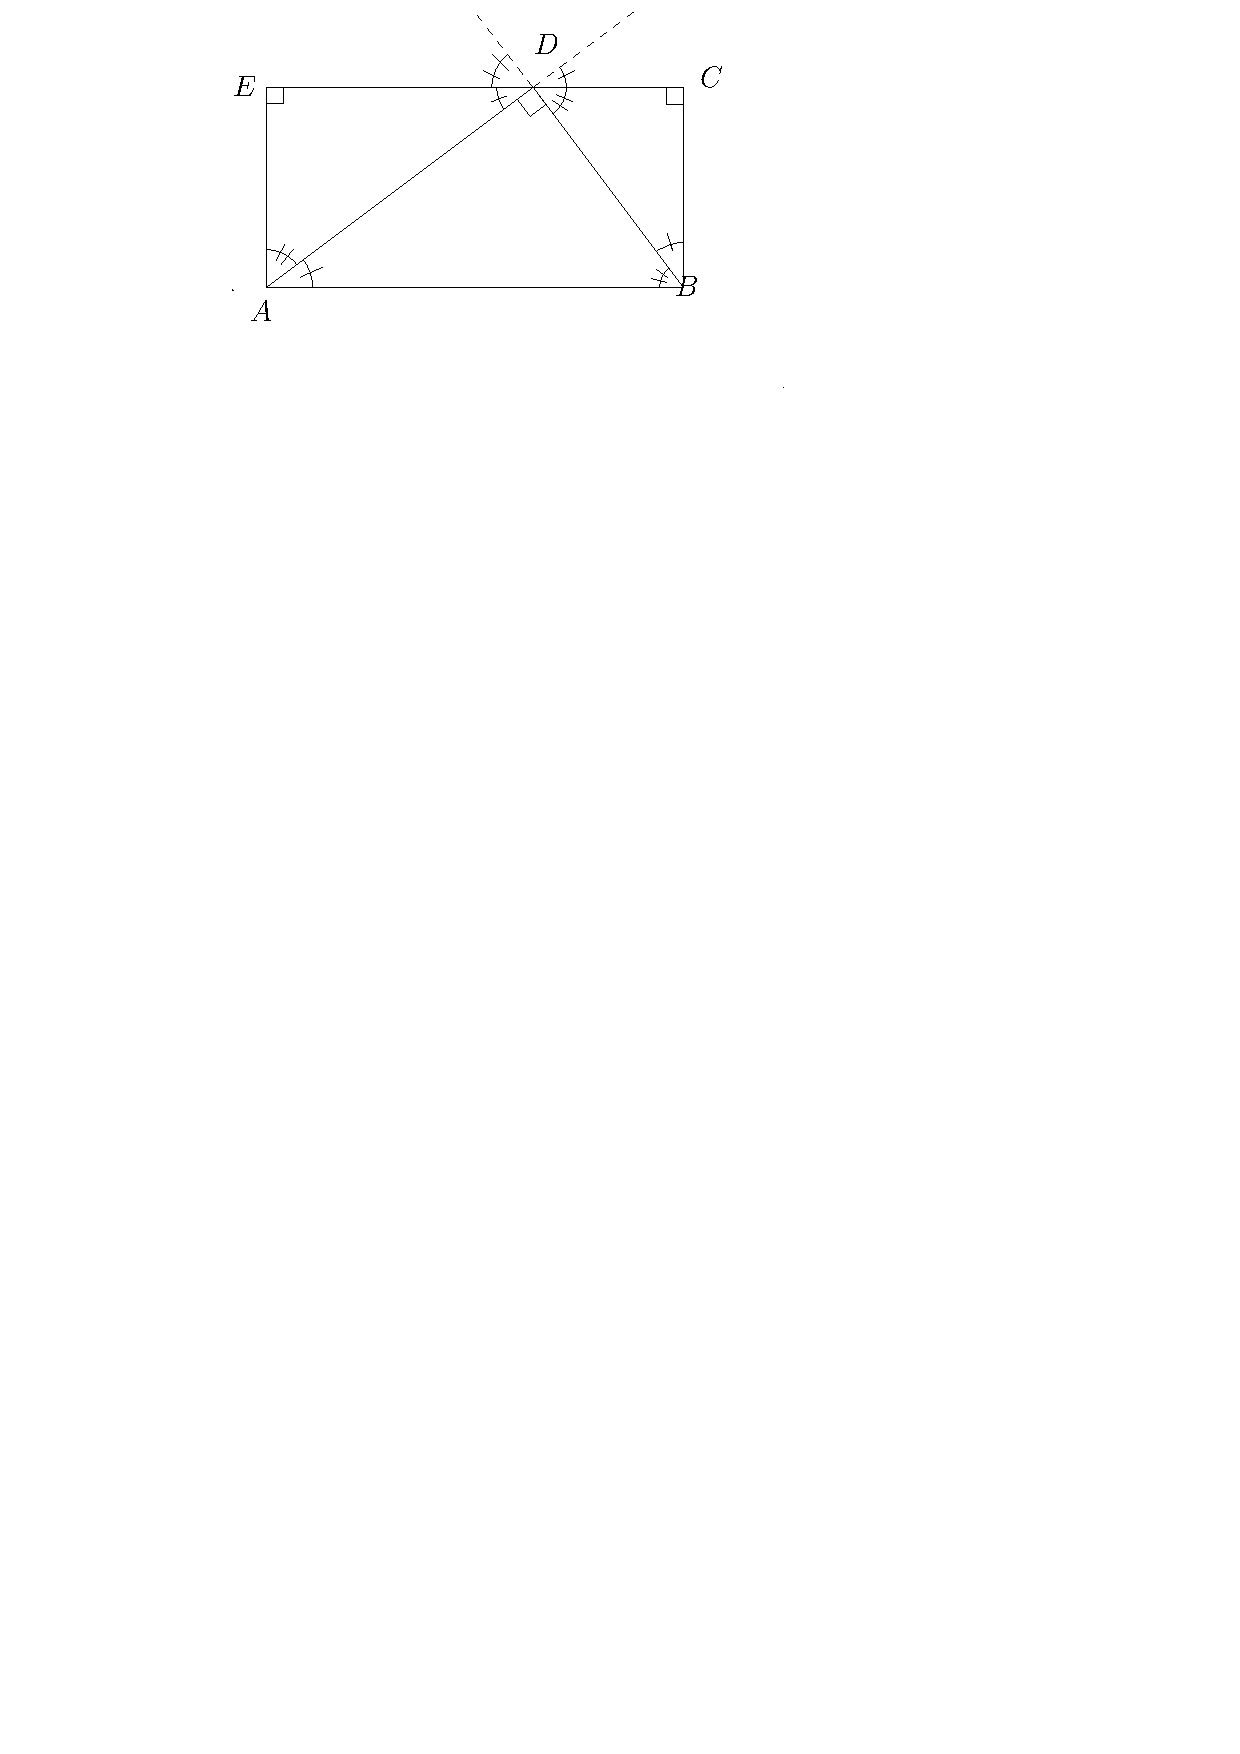
\includegraphics[clip,trim = 0.5cm 23cm 0.5cm 0cm, width = 0.85\linewidth]{figs/del1_oppg7b.pdf}
		\label{fig:del1_oppg7b}
	\end{figure}
	
	Siden summen av vinklene i en trekant er $180$, vet vi at $\angle BAD + \angle  ABD ? \ang{90}$, og dermed vet vi også at $\angle ADE + \angle BDC = \ang{90}$. Vi har da at $\angle EDC  = \ang{180}$, og dermed må punktene E, D og C ligge på samme linje.
	
	# Fra oppgaven over har vi at $\angle DAE + \angle BAD = \ang{90}$ og at $\angle DBA + \angle CBD = \ang{90}$. Da har vi at alle hjørnene i firkanten vår er $\ang{90}$, altså har vi et rektangel. 
	
	I et rektangel vet vi at parallelle sider er like lange, det vil si at lengden av siden EC skal være lik lengden av siden AB. Altså: $a^2 + b^2 = c^2$, som er Pytagoras' setning.
	
\end{easylist}
\newpage


\section*{Del 2 - med hjelpemidler}

\subsection*{Oppgave 1}
\begin{easylist}[enumerate]
	\ListProperties(Style2*=,Numbers=a,Numbers1=l,FinalMark={)})
	
	# Først husker vi at vinkelen i en sirkel er $\ang{360}$. Vi har en sentralvinkel i figuren, nemlig u. Siden vinkelen i sirkelen må være $\ang{360}$ vet vi derfor at "resten" av vinkelen i sirkelen må være $\ang{360} - u$, siden da blir summen av de to vinklene lik $\ang{360}$. $\angle DCB$ spenner over buen BC, det samme gjør sentralvinkelen vi nettopp fant, $\ang{360} - u$. Vi vet at periferivinkler som spenner over samme bue som en sentralvinkel vil være halvparten så stor som sentralvinkelen. Dermed har vi $$\angle DCB = \frac{1}{2} \cdot (\ang{360} - u) \\ = \ang{180} - \frac{1}{2}u$$.
	
	Altså har vi vist at $\answer{\angle DCB = \ang{180} - \frac{1}{2}u}$
	
	# Fra oppgave a) vet vi at $\angle DCB = \ang{180} - \frac{1}{2}u$. $\angle BAD$ er en periferivinkel som spenner over samme sirkelbue som sentralvinkelen $u$, derfor vet vi at  $\angle BAD = \frac{1}{2}u$. Legger vi nå sammen disse to vinkelene får vi:
	
	$$\angle BAD + \angle DCB = \ang{180} - \frac{1}{2}u + \frac{1}{2}u = \ang{180}$$
	
	Videre er summen av vinkler i en firkant $\ang{360}$, derfor vet vi at $\angle CBA + \angle ADC = \ang{180}$
	
	Dermed har vi vist at $\angle BAD + \angle DCB = \angle CBA + \angle ADC = \ang{180}$.
	
	
\end{easylist}
\subsection*{Oppgave 2}

\begin{easylist}[enumerate]
	\ListProperties(Style2*=,Numbers=a,Numbers1=l,FinalMark={)})

	Likningen for en sirkel kan skrives $$x^2 + y^2 + ax + by + c = 0$$, og vi får oppgitt at $A(3,8)$, $B(9,6)$ og $C(13,-2)$ ligger på sirkelperiferien. 
	
	# For at likningen skal gjelde for en sirkel som går gjennom alle de gitte punktene, må likningen gå opp uansett hvilket punkt vi setter inn i likningen. For å finne et likningssystem som svarer til det over, setter vi altså inn $x$- og $y$-koordinatene for hvert av punktene i hver sin likning. Likningssystemet blir da:
	
	\begin{equation*}
		\begin{cases} 3^2 + 8^2 + 3a + 8b + c = 0
		\\ 9^2 + 6^2 + 9a + 6b + c = 0 
		\\ 13^2 + (-2)^2 + 13a - 2b + c = 0 
		\end{cases}
	\end{equation*}
	
	# Vi skriver inn hver likning i CAS, markerer alle linjene og trykker på x=. Vi kan også bruke kommandoen Løs, og skrive inn hvilke linjer CAS skal løse. Dette ville vi i mitt tilfelle gjort slik: Løs(\{\$1,\$2,\$3\}).

	\begin{figure}[ht!]
		\centering
		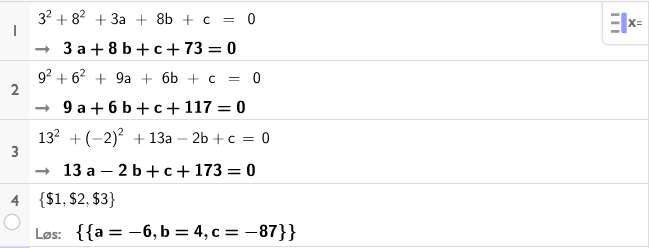
\includegraphics[width = 0.85\linewidth]{figs/del2_oppg2.png}
		\label{fig:del1_oppg7}
	\end{figure}

\end{easylist}


\subsection*{Oppgave 3}
\begin{easylist}[enumerate]
	\ListProperties(Style2*=,Numbers=a,Numbers1=l,FinalMark={)})
	
	# For at vi i denne situasjonen skal kunne bruke en binomisk sannsynlighetsmodell må vi anta at alle delforsøkene er uavhengige. Det vil i praksis si at dersom flere reiser sammen, så vil fremdeles alle i reisefølget møte opp eller ikke uavhengig av hva de andre i gruppen gjør.
	
	# Her kan vi bruke sannsynlighetskalkulatoren i GeoGebra. Siden flyet har plass til maks 116 passasjerer, må vi altså undersøke hva sannsynligheten er for at 116 passasjerer eller mindre møter opp når selskapet har solgt 122 billetter. I sannsynlighetskalkulatoren legger vi da inn $n = 122$, $p = 0.94$ og $P(X \leq 116)$. Resultatet blir da:
	
	\begin{figure}[ht!]
		\centering
		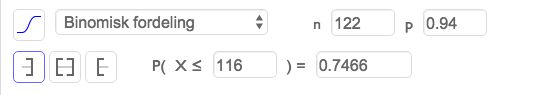
\includegraphics[width = 0.85 \linewidth]{figs/del2_oppg3b.png}
		\label{fig:del2_oppg3b}
	\end{figure}
	
	\answer{Sannsynligheten for at alle som møter får plass på flyet er 74.7\%}

	# Siden vi skal finne ut hvor mange billetter selskapet kan selge, er det altså $n$ i denne oppgaven vi må bestemme. Da lar vi fremdeles $p = 0.94$, $P(X \leq 116)$, og så tester vi for hvilke verdier av $n$ som gjør at sannsynligheten vi får ut blir $\geq 95\% $. Vi vet fra oppgaven over at de ikke kan selge 122 billetter, for da blir sannsynligheten for at alle får plass for liten i forhold til hva selskapet øker. Derfor kan vi prøve å sette inn for eksempel $n = 120$
	
	
	
	\begin{figure}[h]
		\centering
		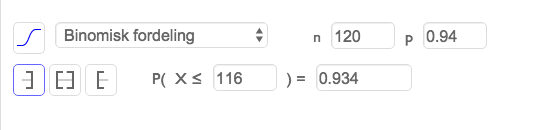
\includegraphics[width = 0.85 \linewidth]{figs/del2_oppg3c1.png}
	\end{figure}
	
	\newpage
	Vi ser at dette antallet også vil gi for liten prosent. Vi prøver da med for eksempel $n = 119$
	
	\begin{figure}[ht!]
		\centering
		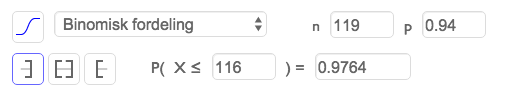
\includegraphics[width = 0.85 \linewidth]{figs/del2_oppg3c2.png}
	\end{figure}
	
	Dette ser vi gir en bedre prosent enn ønskelig, så flyselskapet kan altså selge 119 billetter og få at sannsynligheten er minst 95 \% for at alle som møter opp får plass på flyet.	
	
	
\end{easylist}

\subsection*{Oppgave 4}

\begin{easylist}[enumerate]
	\ListProperties(Style2*=,Numbers=a,Numbers1=l,FinalMark={)})
	
	# Her må vi først finne ut hvor lange sidene $s$ er som funksjon av x. Da kan vi først se på trekant ABE. Denne er likebeint, så vi vet at den rette linjen fra E ned til linjen AB vil danne $\ang{90}$ med linjen AB, og den vil dele AB i to like store deler. Vi får altså to $\ang{90}$ trekanter, og da kan vi bruke Pytagoras' setning. 
	
	Den ene kateten vil da være halvparten av AB $ = \frac{10}{2}$, mens den andre må vi lete litt mer etter.
	
	Vi ser at høyden i hele firkanten er 10, og at det er en lik trekant som ABE helt øverst i figuren også. Det vil si at vi kan dele denne trekanten opp på samme måte som ABE og få en høyde også her. Vi ser da av figuren at høydene i de to trekantene til sammen er $10-x$, og da vil høyden i hver av trekantene være $\frac{10-x}{2}$. Da har vi altså begge katetene og kan bruke Pytagoras' setning til å finne s.
	
	\begin{equation*}
	\begin{aligned}
		s^2 &= \left (\frac{10-x}{2} \right)^2	+ \left(\frac{10}{2} \right)^2 \\
		 & = \sqrt{\left (\frac{10-x}{2} \right)^2 + \left(\frac{10}{2} \right)^2} \\
		 & = \sqrt{\frac{(10-x)^2}{4} + \frac{10^2}{4}} \\
		 & = \frac{1}{2} \sqrt{(10-x)^2 + 10^2} \\
		 & = \frac{1}{2} \sqrt{(x-10)^2 + 10^2} 		
	\end{aligned}
	\end{equation*}
	
	Den totale strekningen er
	
	\begin{equation*}
		\begin{aligned}
			g(x) & = x + 4s \\
			& = x + 4 \cdot  \frac{1}{2} \sqrt{(x-10)^2 + 10^2} \\
			& = \answer{x + 2\sqrt{(x-10)^2 + 10^2}}
		\end{aligned}	
	\end{equation*}
	
	
	# Denne oppgaven kan gjøres på forskjellige måter i CAS. Her har jeg valgt å først skrive inn funksjonsuttrykket for g, deretter derivere dette, og finne ut når den deriverte er $0$ ved å bruke kommandoen nullpunkt. Deretter sjekket jeg hva den andrederiverte var i dette punktet. Siden den andrederiverte var større enn $0$, vet vi at punktet vi fant er et bunnpunkt.
	
	
	\begin{figure}[ht!]
		\centering
		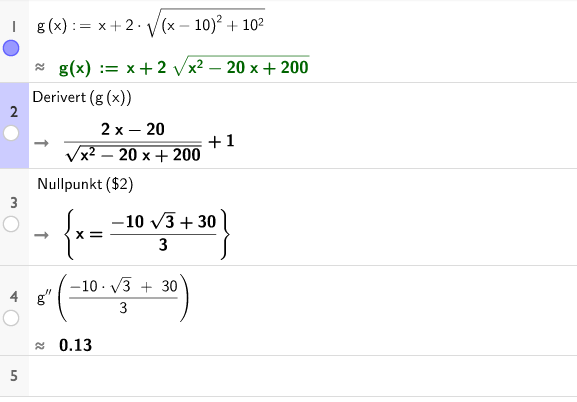
\includegraphics[clip, trim= 0cm 0cm 0cm 0cm, width = 0.70 \linewidth]{figs/del2_oppg4b.png}
	\end{figure}
\end{easylist}

\subsection*{Oppgave 5}

\begin{easylist}[enumerate]
	\ListProperties(Style2*=,Numbers=a,Numbers1=l,FinalMark={)})
	
	# Bruker kommandoen "Kurve(Uttrykk,Utrykk, Parametervariabel, start, slutt)".
	\begin{figure}[ht!]
		\centering
		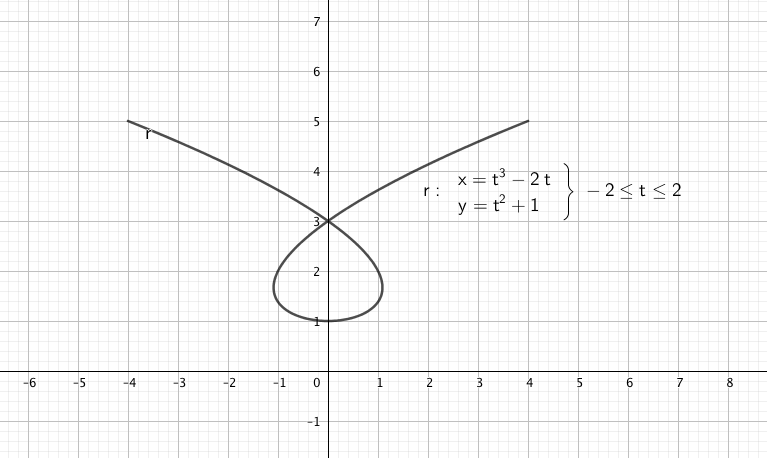
\includegraphics[width = 0.85\linewidth]{figs/del2_oppg5a.png}
	\end{figure}
	
	# Fartsvektoren er den deriverte av posisjonsvektoren.
	
	\begin{equation*}
		\begin{aligned}
			\vec{v}(t) & = \vec{r}'(t) & = [3t^2 -2, 2t] \\
			\vec{v}(-1) & = [3(-1)^2,2(-1)] \\
			& = [3-2,-2] \\
			& = [1,-2] 
		\end{aligned}
	\end{equation*}
	
	Videre har vi at banefarten er $$|\vec{v}(t)| = \sqrt{1^2 + (-2)^2} = \sqrt{1 + 4} = \sqrt{5}$$.
	
	For å tegne inn denne vektoren i graftegneren bruker jeg kommandoen "Vektor(startpunkt, sluttpunkt)". Jeg vet at startpunktet skal være i $\vec{r}(-1)$, og vet at sluttpunktet vil være der $\vec{v}(-1)$ slutter dersom jeg starter i dette punktet, altså i $\vec{r}(-1) + \vec{r}'(-1)$.

	\begin{figure}[ht!]
		\centering
		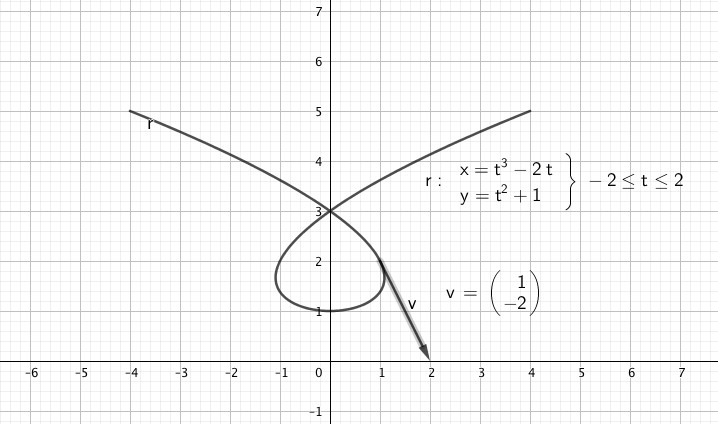
\includegraphics[clip, trim= 0cm 0cm 0cm 3cm, width = 0.85\linewidth]{figs/del2_oppg5b.png}
	\end{figure}
	
	\newpage
	# Dette kan gjøres på flere måter. Her har jeg valgt å først definere formelen for banefarten. Deretter løser jeg v = 2. 
		\begin{figure}[ht!]
			\centering
			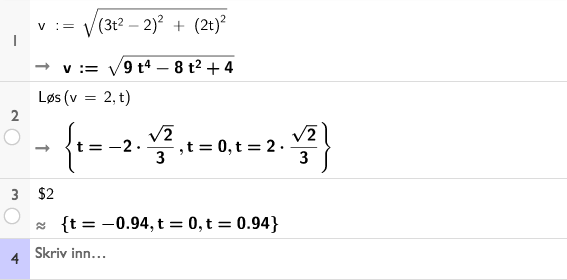
\includegraphics[width = 0.85\linewidth]{figs/del2_oppg5c.png}
		\end{figure}
		
		# Denne oppgaven kan også fint løses i CAS med samme tankegang som brukes under. Først finner vi akselerasjonsvektoren. Dette er den deriverte av fartsvektoren. Deretter sjekker jeg for hvilke $t$-verdier som gjør at skalarproduktet mellom de to vektorene er 0. Dette gjør vi fordi vi vet at hvis skalarproduktet mellom to vektorer er 0, må vinkelen mellom dem være $\ang{90}$. 
		
		$$\vec{a}(t)  = \vec{v}(t)  = [6t,2] $$
		
		\begin{equation*}
			\begin{aligned}
				\vec{a}(t) \cdot \vec{v}(t) &= 0 \\
				[3t^2 -2,2t] \cdot [6t,2] & = 0 \\
				(3t^2 - 2) \cdot 6t + 2t \cdot 2  & = 0\\
				18t^3 - 12t + 4t & = 0 \\
				18t^3 - 8t & = 0 \\
				2t(9t^2 -4) & = 0 \\
			\end{aligned}
		\end{equation*}
		
		Da får vi enten $t = 0$ eller $9t^2 = 0$. Vi må løse siste likning også for t.
		
		\begin{equation*}
			\begin{aligned}
				9t^2 -4 & = 0 \\
				9t^2 & = 4 \\
				t^2 & = \frac{4}{9}\\
				t &= \pm \sqrt{\frac{4}{9}} \\
				t &= \pm \frac{2}{3}
			\end{aligned}
		\end{equation*}
		
		De to vektorene står altså vinkelrett på hverandre når $t = 0$ og når $t = \pm \frac{2}{3}$.
		
		Deretter sjekker vi når banefarten får sine ekstremalpunkter. Dette gjør vi ved å derivere banefarten og se når denne er lik 0.
		
		\begin{equation*}
			\begin{aligned}
				|\vec{v}(t)| & = \sqrt{(3t^2 - 2)^2 + (2t)^2} \\
								 & = \sqrt{9t^4 - 12t + 4 +4t^2} \\
								 & = \sqrt{9t^4 - 8t^2 + 4}\\
								 & = (9t^4 - 8t^2 + 4)^{\frac{1}{2}} \\
				|\vec{v}(t)| ' &= \frac{1}{2} \cdot (9t^4 - 8t^2 + 4)^{-\frac{1}{2}} \cdot (36t^3 -16t) \\
								& = \frac{18t^3 - 8t}{\sqrt{9t^4 - 8t^2 + 4}} \\
			\end{aligned}
		\end{equation*}
		
		Den deriverte er 0 når telleren er 0.
		
		\begin{equation*}
			\begin{aligned}
				18t^3 - 8t & = 0 \\
				2t(9t^2 -4) & = 0 \\
			\end{aligned}
		\end{equation*}
		
		Dette ser vi er akkurat samme likning som vi hadde lengre oppe. Dermed vil løsningene være de samme. 
		
		Dermed har vi vist at banefarten har sine ekstremalpunkter i de punktene der fartsvektoren står normalt på akselerasjonsvektoren.
		
	
\end{easylist}




\end{document}